
\documentclass[
	%print, % Uncomment to convert colors to CMYK for printing purposes
	%a1papersize, % Uncomment to use an A1 paper size instead of the default A0 paper size
]{ImperialPoster}
\usepackage{helvet}
\usepackage{wrapfig}
\usepackage{placeins}

\postertitle{Improving visible light transmittance of Starch-Gelatine films through the addition of papaya and cantaloupe pur\'{e}e}  % produces ée} % The poster title, can be split across multiple lines manually with \\

% Contributor/author names, can be split across multiple lines manually with \\
% Add affiliations using the \affiliation{} command
\posterauthors{Douglas Penning\affiliation{1},\\ Alvin Zhu\affiliation{1},\\ Gabriel Yang\affiliation{1},\\ Manjula Silva\affiliation{1}}

%----------------------------------------------------------------------------------------

\begin{document}

\newpage

\titlesection % Output the title section, automatically populated using the information in the POSTER INFORMATION block above

\begin{multicols}{2} % Start the three-column layout
	
\section{Motivation}

    

    \begin{minipage}{0.4\linewidth}
        \centering
        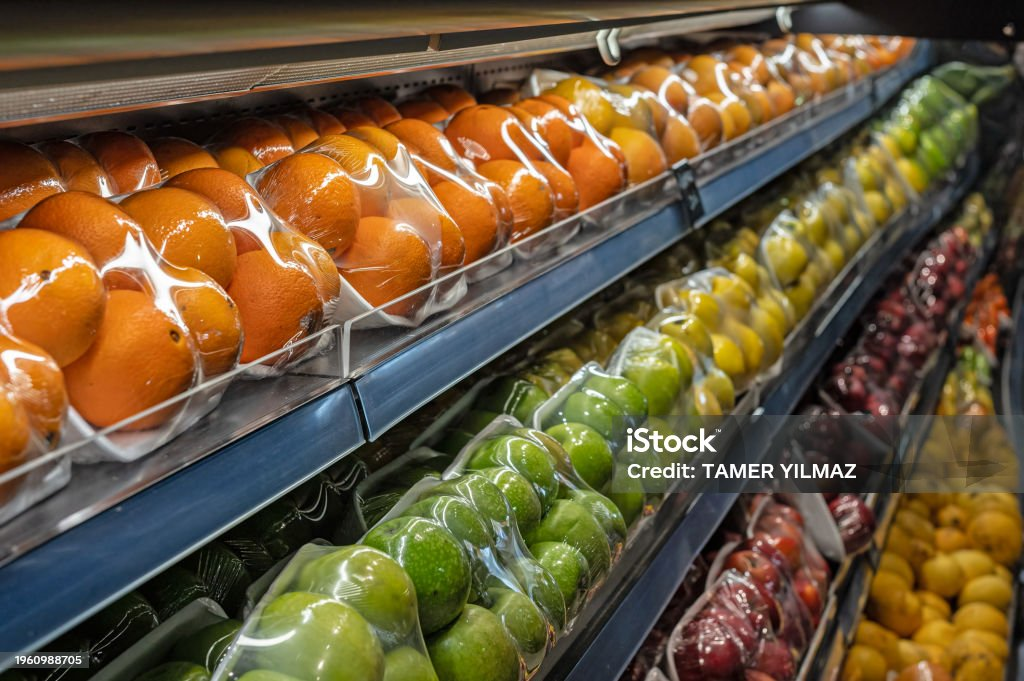
\includegraphics[width=\linewidth]{PLACEHOLDER.jpg}
    \end{minipage}%
    \begin{minipage}{0.5\linewidth}
    \centering
    \begin{quote}
    \textcolor{ICLDarkBlue}{
    		"23 \% of all Polyethylene film use is for food packaging applications" \textsuperscript{[1]}}
	\end{quote}
    \end{minipage}
    
            Concerns over widespread use of petroleum-based packaging have driven interest in biodegradable starch-gelatine films.
            Transparency of these sustainable alternatives, may be improved through the use of papaya and cantaloupe purée additives.
    

\section{Materials \& Methodology}	

    	\begin{figure}[H] % [H] forces the figure to be output where it is defined in the code (it suppresses floating)
        \centering
		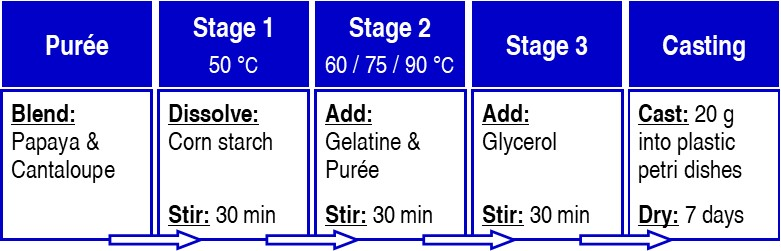
\includegraphics[width = 0.85\linewidth]{Flow.jpg} % Figure image
	\end{figure}	


       
   

        \begin{table}[H] % [H] forces the table to be output where it is defined in the code (it suppresses floating)
        \centering
        \fontsize{0.6\normalbaselineskip}{0.6\normalbaselineskip}\selectfont
		\begin{tabular}{L{0.4\linewidth} C{0.4\linewidth}}
			\toprule
			\textbf{Component} & \textbf{Quantity} \\
			\midrule
		      Corn starch\textsuperscript{2} & 2 wt. \%\\
			Gelatine\textsuperscript{2} &   6 wt. \%\\
		      Papaya OR Cantaloupe\textsuperscript{1} & 9 - 18 wt. \%\\
            Glycerol\textsuperscript{2} & 6 wt. \%\\
            Deionised Water & q.s. \\
			\bottomrule
		\end{tabular}
	\end{table}
     \smalltext{\textsuperscript{1} Waitrose \& Partners (Brazil), \textsuperscript{2} Sigma-Aldrich}

	
	\section{Results}
    
    \textcolor{ICLBlue}{Visible light transmittance} ($\lambda$ = 500 nm) was found to \textbf{increase above 13 wt. \% papaya} loadings and appears to be strongly correlated. High papaya loadings reduced particulate count, potentially due to reduced hydrogen bonding between starch-gelatine thus reducing scattering.  
    
    \begin{figure}[H] 
    \centering
		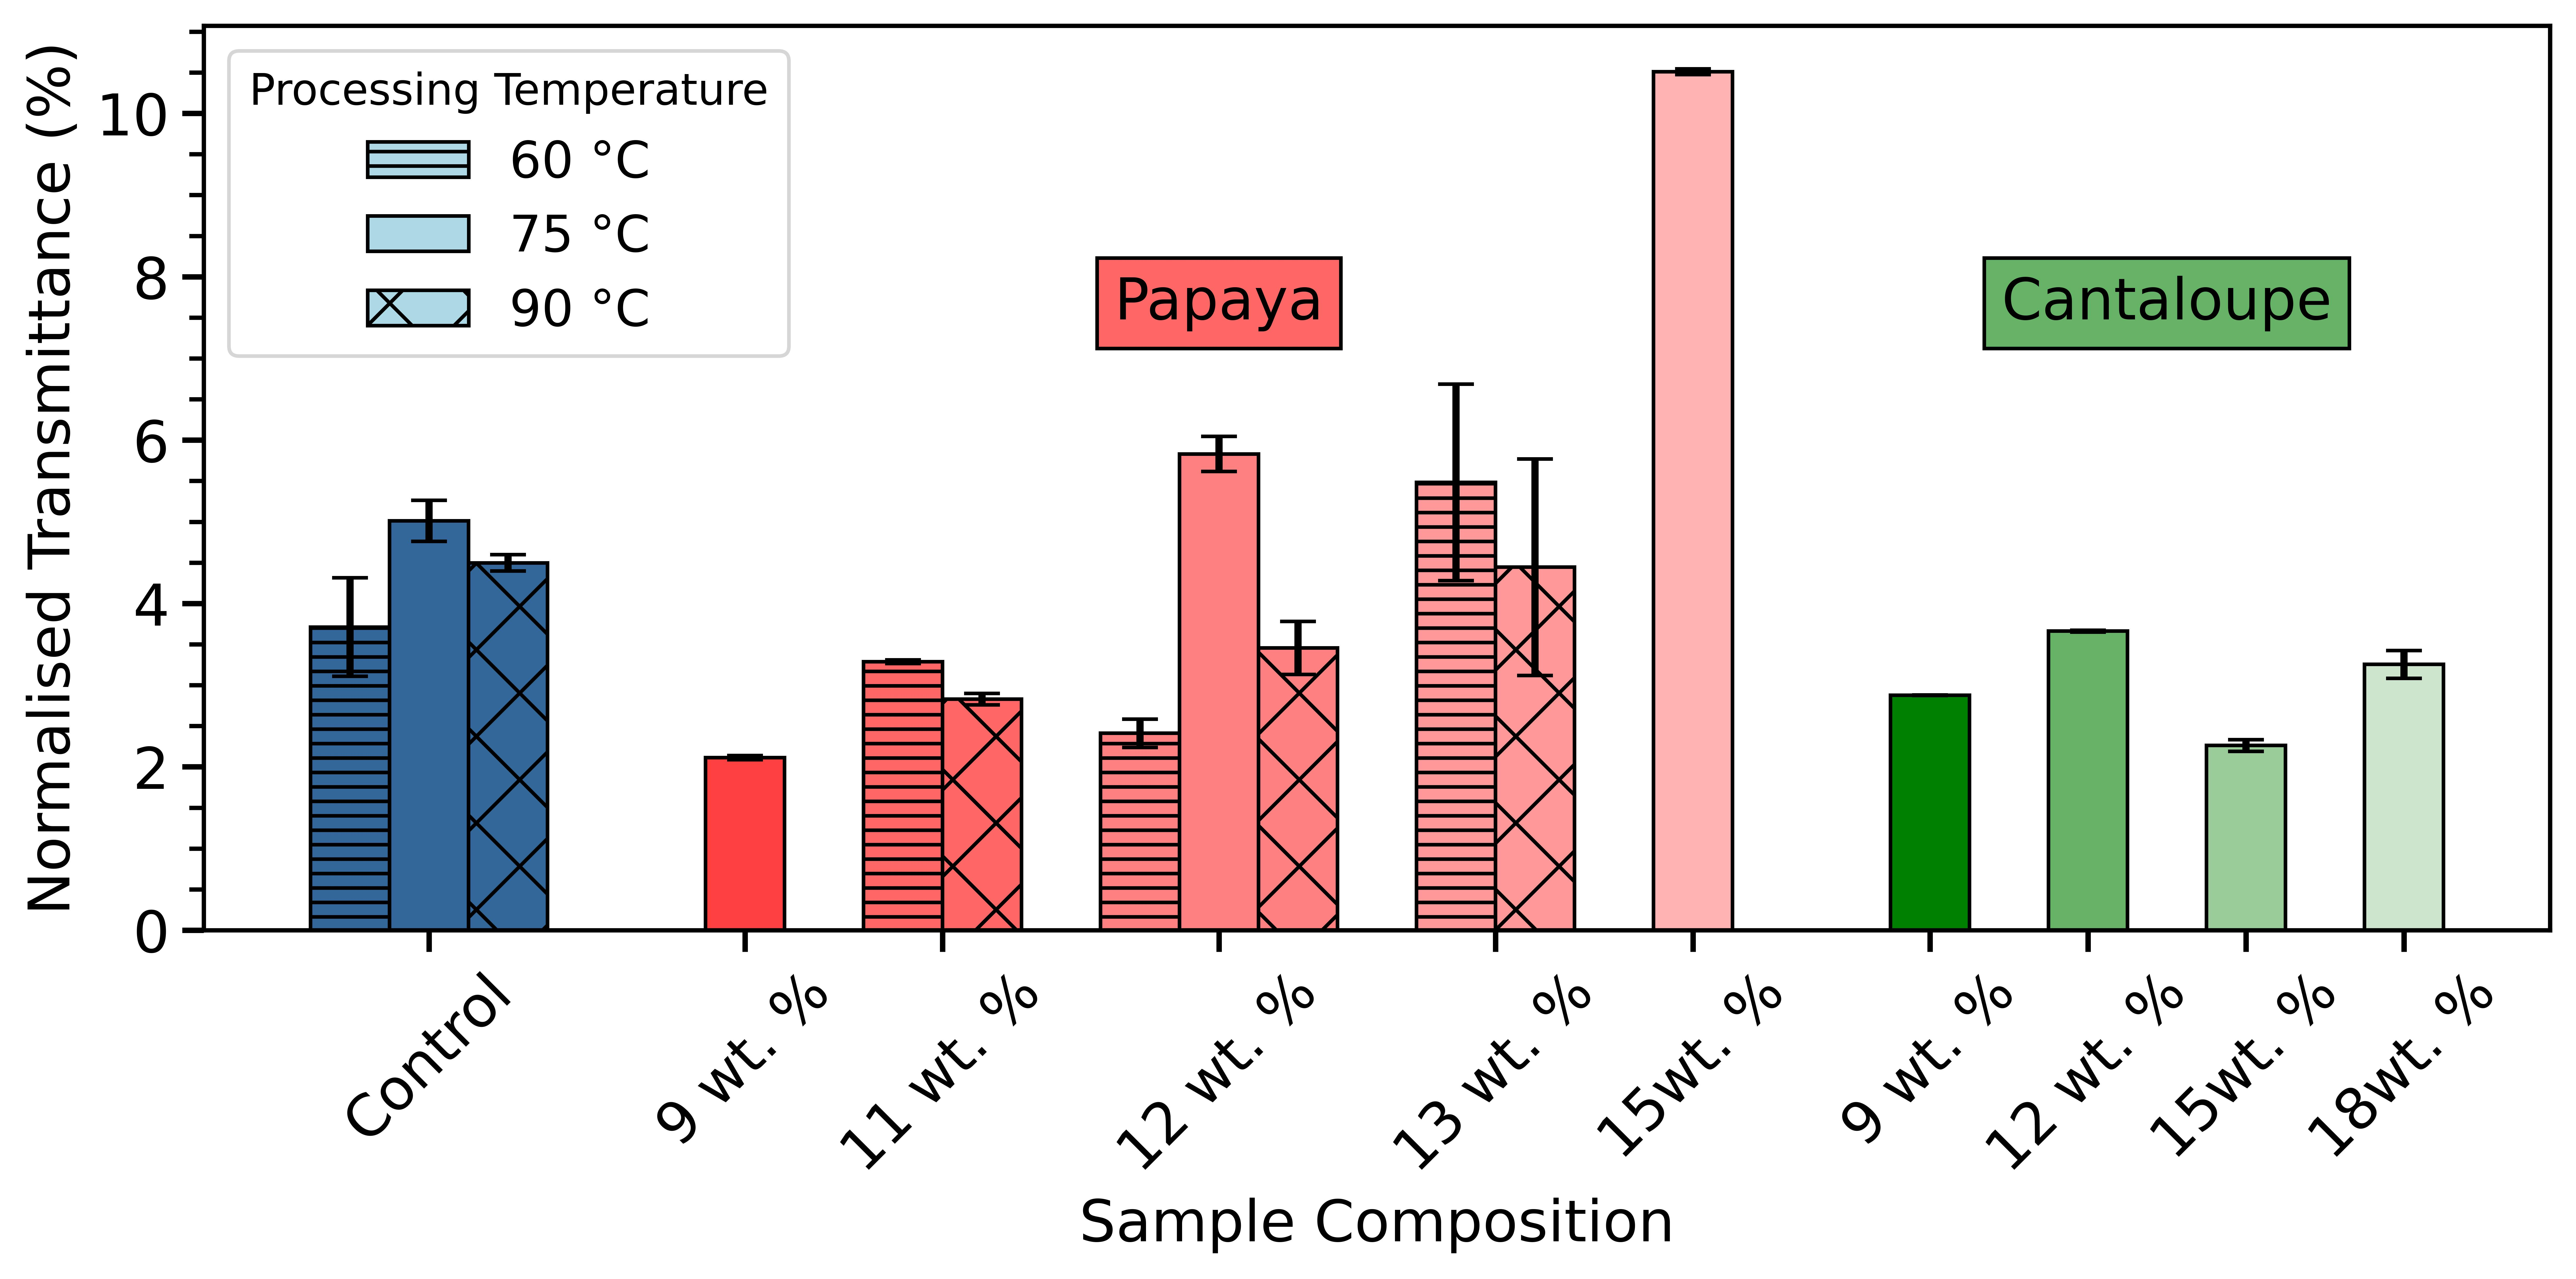
\includegraphics[width=0.98\linewidth]{UVVIS_2C.jpg} % Figure image
		\caption{Normalised average visible light transmittance taken at $\lambda$ = 500 nm via ASTM D1746-15 standard, for all samples. Error bars show standard deviation between repeats.}
	\end{figure}	

	\vspace{-10mm}
	
	
    \textcolor{ICLBlue}{Water contact angle} rose with low papaya content but decreased at higher pur\'{e}e levels. All films were found to \textbf{remain hydrophilic} ($\theta$ < 90°). Sugars promote hydrogen bonding and reduce crystallinity thus increasing wettability.

    \columnbreak
     Rougher air-facing surfaces enhanced hydrophilicity via the Wenzel effect \textsuperscript{[2]}. \textbf{High processing temperatures increased hydrophobicity.}

    \begin{figure}[H] 
    \centering
    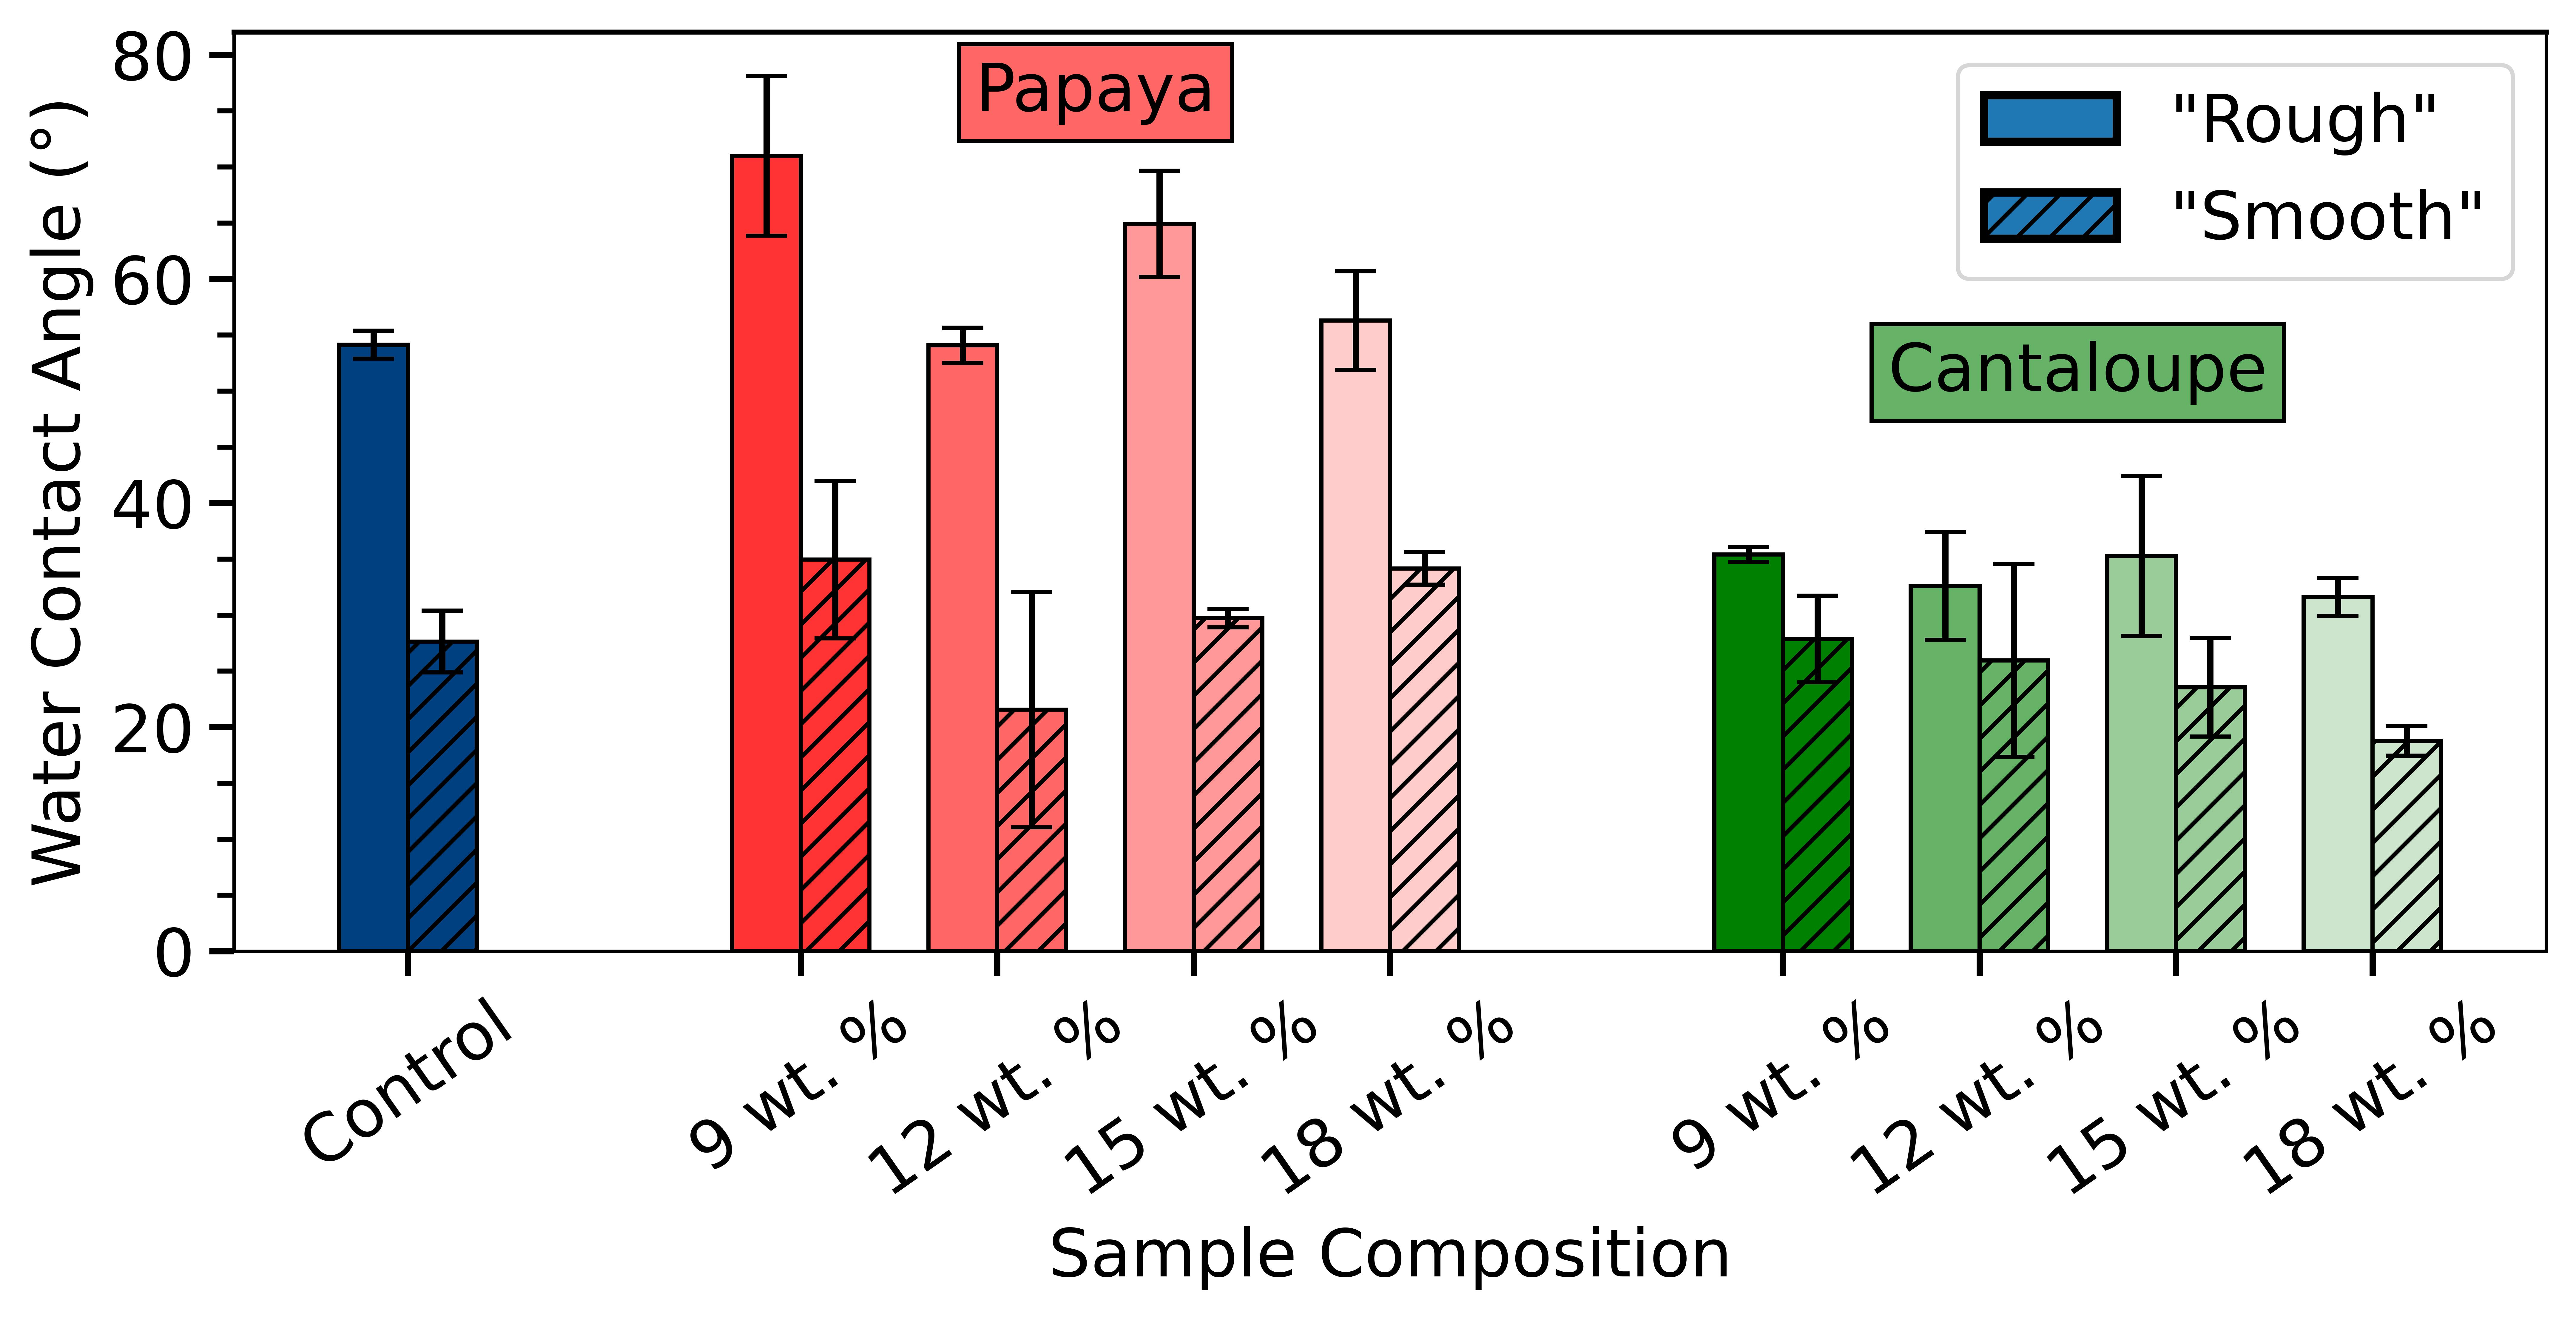
\includegraphics[width=0.95\linewidth]{CA_2C.jpg} % Figure image
    \caption{\textbf{(Above)} Water contact angle (°) measured via sessile drop for samples produced at a Stage 2 temperature of 75 $^{\circ}$C. Error bars represent standard error between repeats. Hatched bars show the “smooth” mould facing side of the film.\\ \\    
    \textbf{Figure 3: (Below)} Elongation at break for polymer samples showing mean values with standard deviation error bars. \textbf{(A)} Samples produced at 75 $^{\circ}$C \& \textbf{B}) Papaya samples produced at 60 and 90 $^{\circ}$C. Measured using ZwickRoell™ z010 at test speed of 10mm/min}
    
	\end{figure}

\vspace{-25mm}
\begin{minipage}{0.55\linewidth}
    \begin{figure}[H] 
        \centering
        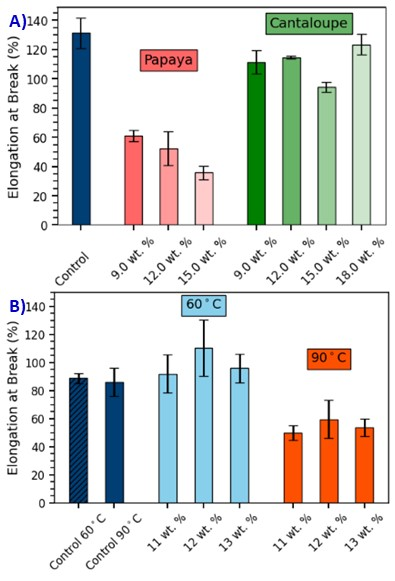
\includegraphics[width=\linewidth]{Tensile_2C.jpg} % Figure image
    \end{figure}
\end{minipage}
\hfill
\begin{minipage}{0.4\linewidth}
\begin{raggedright}
    \hyphenpenalty=10000
    \exhyphenpenalty=10000
    Papaya loading significantly reduced \textcolor{ICLBlue}{mechanical performance}, while cantaloupe had minimal impact on Young’s modulus (\textit{E}), elongation at break (\textit{EAB}), and tensile strength (\textit{TS}).

    \vspace{45mm}

    Higher processing temperature notably decreased \textit{EAB} (except Controls) indicating changes to the papaya composition. 

\end{raggedright}
\end{minipage}
	

    \vspace{-15mm}
    \section{Conclusion}
    \vspace{-5mm}
	
	\largepercent{\textasciitilde 110 \%} increase in transmittance at \(\lambda\) = 500 nm
    
	  \begin{itemize}
      \item Papaya ≥13 wt.\% improves transparency at 500 nm
      \item Pure\'{e}s reduce \textit{TS} and \textit{EAB}; low cantaloupe increases \textit{E} by \textbf{22 ± 57 \%}.
      \item Higher processing temperatures lower \textit{EAB} by \textbf{35.6 ± 12.7 \%}.

    \end{itemize}

\vspace{-1.2\baselineskip}

\begin{center}
  \textcolor{ICLBlue}{\rule{\linewidth}{0.2pt}} % top line
  \vspace{1mm}
  \textcolor{ICLBlue}{\textbf{Summary:}} Demonstrated a clear improvement in film optical performance, though further optimisation is still needed.
  \vspace{1mm}
  \textcolor{ICLBlue}{\rule{\linewidth}{0.2pt}} % bottom line
\end{center}



\vspace{-1.2\baselineskip}
\textbf{\textcolor{ICLBlue}{ Future research:}}  Refine drying protocols and explore hybrid pur\'{e}e blends.
  
	
	
	\subsection{Affiliations}
	
	% Affiliation institutions, the first parameter is the affiliation number (matching the author list) and the second is the institution
	\affiliationentry{1}{Department of Materials, Imperial College London}\\
    \hspace{1mm}

\vspace{-1.2\baselineskip}
\smalltext{
    \textsuperscript{[1]} “Database - Eurostat” https://ec.europa.eu/eurostat/data/database \\
    \textsuperscript{[2]} "Citation xyzabc"\\
    \textsuperscript{[2]} "Citation xyzabc"\\

}

\end{multicols}
\end{document}
